%!TEX root = ../thesis.tex

\chapter{Background}
\label{ch:background}

In this chapter we describe existing technology that will be referred to throughout the paper.

\section{GitHub}

In this section we explore the pull request and issue features of GitHub.

\subsection{Issues}

GitHub issues is a useful feature for tracking, discussing and logging various issues/problems on a GitHub repository.
Any collaborator to a repository may open a GitHub issue, and describe any problem, idea or issue they have.
Other users may then contribute to the issue by commenting on it, easing the communication process within a project.
GitHub issues can therefore function as a discussion hub, and makes it especially useful for larger projects involving several people. 

\begin{figure}[ht]
    \centering
    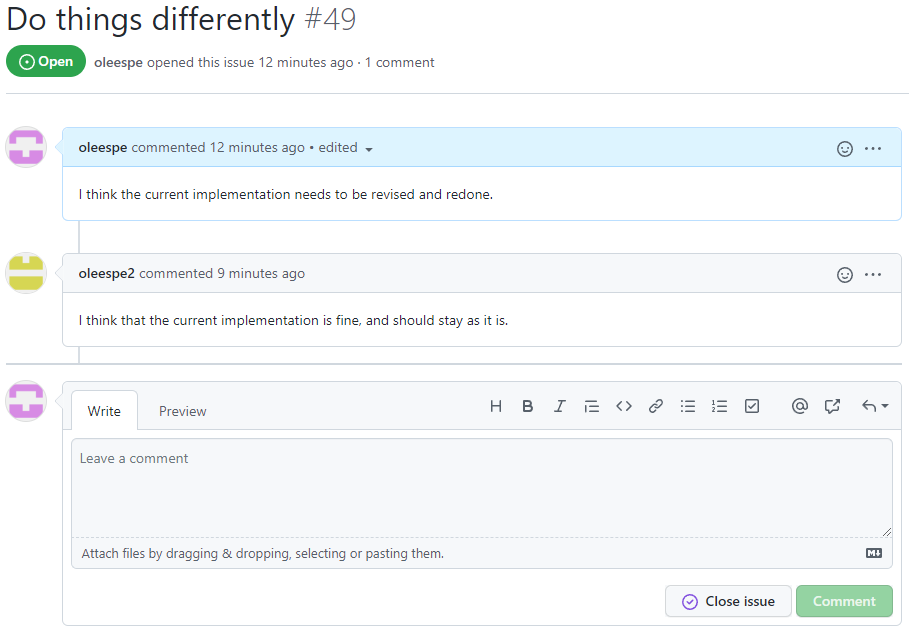
\includegraphics[width=\textwidth]{photos/github-issue.PNG}
    \caption{Example of a GitHub issue comment section}
    \label{fig:github-issue}
\end{figure}

\subsection{Pull requests}

Pull requests are a desire to merge any feature branch, into the main branch of a repository.
GitHub supports managing pull requests through its user interface, and allows any contributor to a repository to create a pull request.
Through the user interface, progress on a branch can be tracked, reviewed and commented on.
In this sense, GitHub pull requests function as a central hub for feature branches.

Code review is also a central part of GitHub pull requests.
Any eligible user may review the source code of a given pull request, and through GitHub's user interface comment and request changes.
The reviewer may also use reviews to approve a pull request for merging.

Pull requests can also be linked to issues.
Doing this will automatically associate any linked issue to the pull request, and cause them to close when the pull request closes.
A common workflow would be to create an issue, describing a problem, and then creating an associated pull request for this issue.

Through its features, GitHub pull requests offer an efficient way of implementing new features to any project.
As well as easing the communication of desired changes to any source code.

\subsection{Workflows}

Maybe maybe

\section{QuickFeed}

\subsection{Introduction}
Only focused on backend

\subsection{Protobuf}

\subsection{gRPC}

\subsection{Running tests on student code}

\subsection{Integration with GitHub}

